%% LyX 2.1.2 created this file.  For more info, see http://www.lyx.org/.
%% Do not edit unless you really know what you are doing.
\documentclass[english]{article}
\usepackage{courier}
\usepackage[T1]{fontenc}
\usepackage[latin9]{inputenc}
\usepackage{geometry}
\geometry{verbose,tmargin=2.5cm,bmargin=2.5cm,lmargin=2.5cm,rmargin=2.5cm}
\usepackage{url}
\usepackage{amsmath}
\usepackage{graphicx}

\makeatletter
%%%%%%%%%%%%%%%%%%%%%%%%%%%%%% Textclass specific LaTeX commands.
\newcommand{\code}[1]{\texttt{#1}}

\makeatother

\usepackage{babel}
\begin{document}

\title{Finding Correlations in MicroBooNE ``Slow Monitor'' History Data}
\maketitle
\begin{abstract}
This short note describes some technical and mathematical issues in
searching for meaningful correlations in time among the histories
of the over 4000 variables in the MicroBooNE monitoring system. Python
code is provided, its usage explained, and some example results discussed.
\end{abstract}
\global\long\def\arctanh{\operatorname{arctanh}}



\section{Summary of the problem}

We have a recorded history of the readings on each variable in the
MicroBooNE slow control and monitoring system. We'd like to see if
there are correlations between certain selected variables and other
variables, perhaps as part of a search for possible causes of a particular
instability or type of event. This should come with an estimate of
the statistical significance of a given correlation.


\section{Quick, the code! Give me the code!}


\paragraph{Where to find the code:}

The Python code is \code{correlator.py} in the \code{correlator}
subdirectory of the Fermilab \code{uboone-slowmon-analysis} Redmine
project. Obtain either by direct download from the web page \url{https://cdcvs.fnal.gov/redmine/projects/uboone-slowmon-analysis/repository},
or by cloning the repository:
\begin{verbatim}
git clone ssh://p-uboone-slowmon-analysis@cdcvs.fnal.gov/cvs/projects/uboone-slowmon-analysis
\end{verbatim}

\paragraph{How to run the code:}

Here is a typical usage:
\begin{verbatim}
import correlator    
c = correlator.Correlator()
corr_data = c.correlate1('uB_TPCDrift_HV01_keithleyPickOff/voltDiff5s60s',
                         60, '2016-02-13 00:00:00', '2016-02-14 00:00:00')
\end{verbatim}
All of the methods of the \code{Correlator} class are documented
with Python docstrings per the usual Pythonic convention. The documentation
as it currently stands is also provided as an appendix to this note.

The arguments to the \code{correlate1} function specify the primary
variable that you want to correlate with all other variables, the
width of time bins in seconds, and the start and stop times. The data
returned is list of \code{(zscore, corr, n, id, name)} tuples, where
\code{zscore} is the estimated number of standard deviations of significance
of the correlation (with sign), \code{corr} is the correlation coefficient,
\code{n} is the number of same-time-bin samples found, \code{name}
is the channel with which the correlation was found, and \code{id}
is the integer identifier used internally by the archiver for the
channel.

The data is initially sorted in order of channel id, but the list
can easily be resorted in order of increasing \code{zscore} by using
Python's sort function.

For plotting the data, I suggest using the PyROOT interface. For example,
the following will plot the histogram of \code{zscore} for all correlation
results where \code{n} is greater than 3.
\begin{verbatim}
import ROOT
h1a = ROOT.TH1F("h1a","z-score distribution",128,-6.4,6.4)
for z in (c[0] for c in corr_data if c[2]>3): 
    h1a.Fill(z)
h1a.Draw()

\end{verbatim}

\paragraph{How to understand the code and its results:}

Please read on.


\section{Theory of operation}


\paragraph{Mathematical and technical issues:}

There is a complication introduced in making correlations by the fact
that the data is asynchronously sampled and recorded. There is also
a technical issue in efficiently retrieving data. With those addressed,
the correlation is fairly straightforward.


\paragraph{Asynchronously sampled data:}

Our EPICS control system samples variables at intervals as short as
0.1~second and as long as an hour; most variables are sampled at
times from a second or two up to a minute. The periodically sampled
data is not synchronized between variables. Some data is pushed in
from other systems at irregular intervals. Furthermore, a new sample
of a variable is only written to the database if it differs from the
previous one by an amount exceeding \code{ADEL}, which is a parameter
is set individually for each variable. The \code{ADEL} parameter
is necessary to avoid filling up the database with meaningless samples,
but the effect is to increase the asynchronicity of the data.

Many ways of dealing with correlations of asynchronously sampled data
can be found in the literature. One of the simplest is to bin the
samples in regular bins in time. This is the approach used in the
example correlator code.

A related question is how to handle cases where two variables do not
both have samples in a given time bin. One possibility is to use interpolation
or simply the previously recorded value of each variable. Assuming
the archiver is working continuously throughout the time interval
of interest, the absence of a sample for a variable implies that the
variable did not change more than its \code{ADEL} since the previous
sample. There are a number of problems with this assumption, however:
a power outage or other problem might cause the archiver to stop working
without recording its shut-down time; \code{ADEL} values for some
channels have been tuned over time, and the archiver does not record
the history of these changes; and we do not know how the value of
the variable varies within $\pm$\code{ADEL} between samples, so
it is not clear whether or how to interpolate between two samples. 

An alternative to interpolating data between samples is to calculate
the correlation of two variables using only time bins where both variables
had samples. This has the effect of increasing the weight of times
where the two variables changed at the same time to within the bin
size, which is not undesirable for the intended application. This
is what is done in the example code.


\paragraph{Database retrieval efficiency:}

The data is stored in a postgresql database. Because of the structure
of the database, it is easy to write SQL queries that take an inordinate
amount of time and server resources to retrieve, but with care the
queries can be made very efficient. It is worth taking a moment to
understand why.

Two tables are important for our purposes: \code{channel} gives the
mapping of channel (variable) names to \code{channel\_id} integers,
and \code{sample} contains all samples recorded for any channel in
a single table of many rows. The \code{sample} table contains fields
\code{channel\_id}, \code{smpl\_time}, \code{nanosecs}, and \code{float\_val}
(among others), giving the channel identifier, the time the sample
was taken, and its value, respectively. The table is indexed by the
key \code{(channel\_id, smpl\_time, nanosecs)}. The result of this
indexing is that it is very efficient to retrieve data for a specified
channel over a range of times in a single request, but very inefficient
to retrieve all channels over a specified time range. It turns out
to be orders of magnitude faster to issue a separate SQL \code{select}
request for each channel than to retrieve all channels over the desired
time in a single request. The SQL \code{group by} clause can be used
to bin the data efficiently at the server before transfer to the client,
which can also improve performance. This approach is used in the \code{correlator}
Python class.


\paragraph{Definition of the correlation coefficient:}

\[
r_{xy}=\frac{\sum_{i=1}^{n}(x_{i}-\bar{x})(y_{i}-\bar{y})}{\sqrt{\sum_{i=1}^{n}(x_{i}-\bar{x})^{2}}\sqrt{\sum_{i=1}^{n}(y_{i}-\bar{y})^{2}}}
\]
where $n$ is the number of samples, $x_{i}$ are the sample values,
$\bar{x}=\frac{1}{n}\sum_{i=1}^{n}x_{i}$ is the mean of $x_{i}$,
and similarly for $y_{i}$ and $\bar{y}$. For reasons explained above,
$n$ is the number of time bins in which both $x$ and $y$ have samples,
and can therefore be different for each pair of variables. Since this
is a number derived from data with random statistical fluctuations,
$r_{xy}$ will itself have random statistical fluctuations.

A special case occurs if either variable has no variance in the sample,
which is guaranteed if $n=1$ but could conceivably happen for any
$n$: in such a case $r_{xy}$ is undefined $(0/0)$. Another special
case occurs when $n=2$ and both variables have variance, in which
case $r_{xy}$ is guaranteed to be exactly $+1$ or $-1$.


\paragraph{Significance score:}

The Fisher transformation\cite{key-1,key-2}
\[
F(r)=\arctanh r
\]
produces a random variable $F(r)$ with an approximately gaussian
distribution, with standard deviation $1/\sqrt{n-3}$ and mean $F(\rho)$,
where $\rho$ is the true correlation of the underlying joint probability
distribution of the two variables. The statistical significance of
a correlation expressed as the number of standard deviations from
zero (also known as standard score or z-score \cite{key-3}) can be
estimated as
\[
z=F(r)\sqrt{n-3}.
\]



\section{Examples}


\paragraph{An example using 1 hour of data in 1-minute bins:}

Here is the distribution of z-score for correlations of the ``blip
detector'' variable \texttt{'uB\_TPCDrift\_HV01\_keithleyPickOff/voltDiff5s60s'}
with every other variable over a 1-hour period, using data binned
in 60-second intervals:

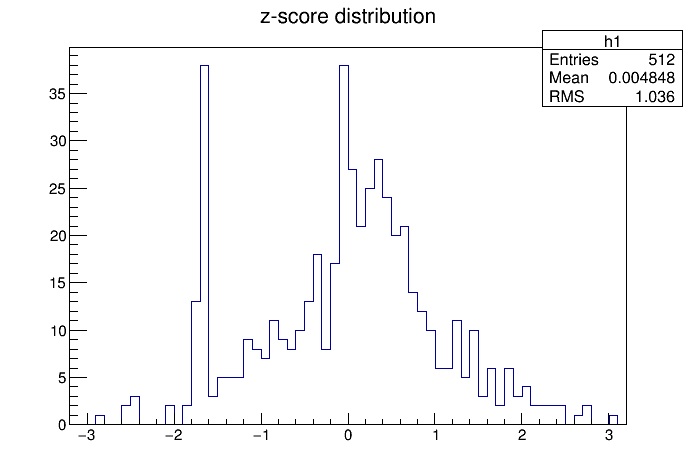
\includegraphics[width=0.9\textwidth]{zscore-dist-1hr-blip}

Only correlations with $n>3$ are histogrammed. The distribution looks
approximately gaussian, and in fact has a mean of zero and an RMS
of 1. But what is that big spike at -1.7? There are almost 40 variables
with the same z-score.

Upon investigation, it turns out that all of those variables increased
continuously with time over the hour in question. (Most of them were
timestamps used for ``age'' calculations.) The value of the ``blip
detector'' happened to trend down over the course of this hour, resulting
in this correlation.

This is not a ``false correlation'' because there is in fact a mathematical
correlation. If this is not the kind of correlation you are looking
for, there are some obvious steps to take, the easiest of which is
to look at data over a longer time range.


\paragraph{An example using 24 hours of data in 1-minute bins:}

Here is the distribution of z-score for correlations of the same ``blip
detector'' variable with all other variables over a 24-hour period,
which includes the 1-hour period above, still using data binned in
60-second intervals:

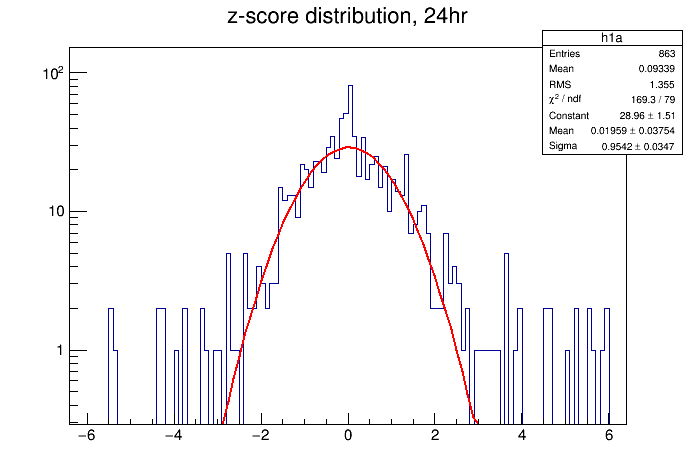
\includegraphics[width=0.9\textwidth]{zscore-dist-24hr-blip}

The spike at $z=-1.7$ has disappeared. The fit function shown in
red is a gaussian; a logarithmic scale is used on the y axis was to
bring out the behavior at large $z$ score. Overall the distribution
is very well approximated by a gaussian, except for an excess at very
small values of $z$ score, and possibly a tail at $|z|>3$.

In my initial look, none of the variables at large $z$ had an obvious
causal relationship with anything related to what the ``blip detector''
is supposed to detect. With over 4000 variables, there are bound to
be some out in the tails of the distribution just from statistics.
However, this does not mean you will not find something interesting
with more data or a different time range. 


\section{Closing thoughts}


\paragraph{Some comments on choice of time bins and time range:}

As seen above, picking a longer time range is a good way to reduce
correlations due to linear trends over a shorter time. Picking a larger
time bin could be a good way to reduce noise and increase sensitivity
to longer-term correlations while reducing sensitivity to short fluctuations.
Picking a smaller time bin could increase sensitivity to fast fluctuations,
but there is the risk of reducing the number of common time-bin samples
with other variables, particularly if the bin size is smaller than
the sampling period for both of the variables.


\paragraph{Some ideas for improvements:}
\begin{itemize}
\item For cases where correlations of fast fluctuations are of primary interest,
a running average or exponentially-time-weighted average of previous
samples could be subtracted from the data to implement a high-pass
filter. 
\item For cases where slow fluctuations are of interest, the opposite could
be done.
\item Linear trends could be subtracted to eliminate the effect seen in
the 1-hour example above, particularly when it is known an interesting
behavior (e.g., a ``blip'') only happened in a particular time range. 
\item The correlator currently only looks for correlations in simultaneous
samples, not correlations with samples earlier or later in time. A
more general cross-correlator could calculate the correlation function.
\end{itemize}
None of the enhancements above would be appropriate for every use
case, but would be appropriate for some, so there should be some way
for the user to select which options are desired.

\appendix

\section{Documentation of correlator module}
\begin{verbatim}
NAME
    correlator

DESCRIPTION
    correlator.py -- implements a correlation-finder for the ControlSystemStudio
    rdb archive engine.
    
CLASSES
    Correlator
    
    class Correlator
     |  Class encapsulating various functions for retrieving data and
     |  calculating correlations.
     |  
     |  Methods defined here:
     |  
     |  __init__(self)
     |      Initialize the correlator -- opens the database on ifdbrep2.
     |      [Currently the host is hard-coded, which should be fixed.]
     |      The smcreader password should be set in the file ~/.pgpass,
     |      which should have mode 0600.
     |  
     |  correlate1(self, channel, dt_s, tstart, tstop)
     |      Get the correlation coefficients of a given channel with
     |      all channels.  channel may be an integer or a string.  dt_s
     |      is in seconds.  tstart and tstop should be time strings in a
     |      format that postgresql understands (ideally ISO8601 / SQL
     |      standard), or a datetime object.
     |      The correlation coefficient calculated is sample-weighted
     |      rather than time-weighted. Only time bins where both variables
     |      have a sample in the same time bin are used.
     |      The data returned is list of (zscore, corr, n, id, name) tuples,
     |      where corr is the correlation coefficient,
     |      n is the number of same-time-bin samples found,
     |      id is the channel id, name is the channel name,
     |      zscore is the number of standard deviations of significance.
     |  
     |  query_timebinned_data(self, channel_id, dt_s, tstart, tstop)
     |      Get data for channel channel_id binned in steps of
     |      dt_s. The channel_id must be an integer.  dt_s is in seconds.
     |      tstart and tstop should be time strings in a format that
     |      postgresql understands (ideally ISO8601 / SQL standard), or
     |      a datetime object.
     |      The data is not fetched.  Use the cursor object to retrieve.
     |      The columns are (channel_id, tbin, avg).

FUNCTIONS
    cor_xy(xdat, ydat)
        Given two sparse lists [(id,xdat),...] and [(id,ydat),...],
        sorted in order of increasing id, find the correlation coefficient
          corr = <dx dy> / (stddev(dx)*stddev(dy))
        using only entries with common ids.
        Returns (corr, n), where corr is as defined above and n is the number of
        samples.  Returns corr=0 if n <= 1.  Meaningless for n <= 2.
    
    test_1()
        A test function for the data retrieval.
        Retrieves all data in a 1-hour period for channels 1 through 4483, 
        one channel at a time.
    
    test_2()
        A test function for the 1-to-all correlation function correlate1().
        Retrieves all data for a 1-day period and finds correlation coefficients
        for correlations of any variable with 
        uB_TPCDrift_HV01_keithleyPickOff/voltDiff5s60s
        and the corresponding z-score significances of the correlations.


\end{verbatim}
\begin{thebibliography}{1}
\bibitem[1]{key-1} Fisher, R.A. (1921). ``On the `probable error' of a coefficient of correlation deduced from a small sample''. Metron 1: 3-32.
  \url{https://digital.library.adelaide.edu.au/dspace/bitstream/2440/15169/1/14.pdf}

\bibitem[2]{key-2}\url{https://en.wikipedia.org/wiki/Pearson_product-moment_correlation_coefficient#Using_the_Fisher_transformation}

\bibitem[3]{key-3}\url{https://en.wikipedia.org/wiki/Standard_score}\end{thebibliography}

\end{document}
